\documentclass[a4paper, 10pt]{article}
\usepackage[utf8]{inputenc}
\usepackage[portuguese]{babel}
\usepackage[pdftex]{graphicx}
\usepackage{geometry}
\usepackage{amsmath}
\usepackage{caption}
\usepackage{xcolor}
\usepackage{hyperref}

\geometry{a4paper, margin=1in}

\title{Modelagem do Pêndulo Simples em \LaTeX \\ Trabalho com Tabelas e Figuras}
\author{Guilherme Turina de Melo | 13679523 | guilhermeturina@usp.br \\ Bárbara Fernandes Dias Bueno | 13679530 | barbarabueno@usp.br}

\begin{document}

\maketitle

\section{Introdução}
O estudo do pêndulo simples é essencial para compreender sistemas dinâmicos, servindo como base valiosa para análises mais complexas, como o pêndulo duplo. Neste relatório, iniciamos nossa exploração pelo pêndulo simples para estabelecer conceitos essenciais antes de nos aprofundarmos no pêndulo duplo.

Exploraremos a derivação das equações de movimento, considerando forças gravitacionais e condições iniciais. A escolha do pêndulo simples proporciona uma base sólida para o entendimento de princípios fundamentais aplicados ao pêndulo duplo.

\section{Modelamento Matemático}
O pêndulo simples é descrito por equações diferenciais que modelam o movimento angular da massa suspensa. Consideramos um pêndulo de comprimento \(L\) com uma massa pontual \(m\) na extremidade.

A equação diferencial que governa o movimento angular \(\theta\) do pêndulo simples é derivada da segunda lei de Newton para rotação:

\begin{equation}
    \frac{d^2\theta}{dt^2} = -\frac{g}{L} \sin(\theta)
\end{equation}

As condições iniciais do problema são \(\theta_0\) (ângulo inicial), \(\omega_0\) (aceleração angular inicial), \(g\) (gravidade), \(L\) (tamanho do fio do pêndulo).

\section{Metodologia Numérica}
Para a análise desse problema, usamos o método de Euler e Euler modificado, com L = 1\,\text{m},\quad g = 9,8\,\text{m/s}^2 
 \(, \theta_0 = \frac{\pi}{4}\) e \(\omega_0 = 0\). Desenvolvemos o método em Python [2] para estudar o problema.

\begin{figure}[h]
    \centering
    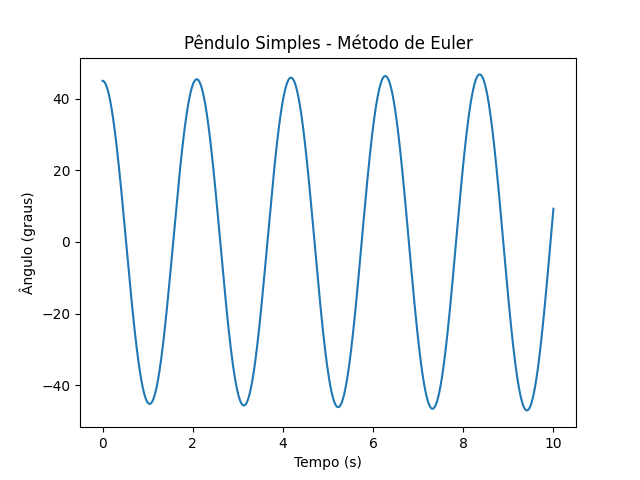
\includegraphics[width=0.6\linewidth]{Figure_PenduloSimples.png}
    \caption{Movimento do Pêndulo Simples.}
    \label{fig:pendulo-simples}
\end{figure}

\section{Resultados}
Os resultados numéricos do método de Euler são apresentados na Tabela \ref{tab:resultados}. Como esperado, o gráfico mostra um movimento harmônico simples. A sensibilidade do método de Euler ao tamanho do passo foi mitigada ajustando o passo para 0,001s.\\

\begin{table}[h]
    \centering
    \begin{tabular}{|c|c|c|}
        \hline
        \textbf{Tempo (s)} & \textbf{Ângulo (Graus)} & \textbf{Aceleração Angular (\( \text{Rad/s}^2 \))} \\
        \hline
        0.00 & 45.00 & 0.0000 \\
        0.50 & 3.01 & -2.3957 \\
        1.00 & -44.83 & -0.3044 \\
        1.50 & -9.05 & 2.3608 \\
        2.00 & 43.88 & 0.6098 \\
        \hline
    \end{tabular}
    \caption{Dados de Resultados do Pêndulo Simples.}
    \label{tab:resultados}
\end{table}

Trabalhando com Euler modificado, obtemos os resultados esperados com passos maiores (0,01s, por exemplo), como mostra a figura:

\begin{figure}[h]
    \centering
    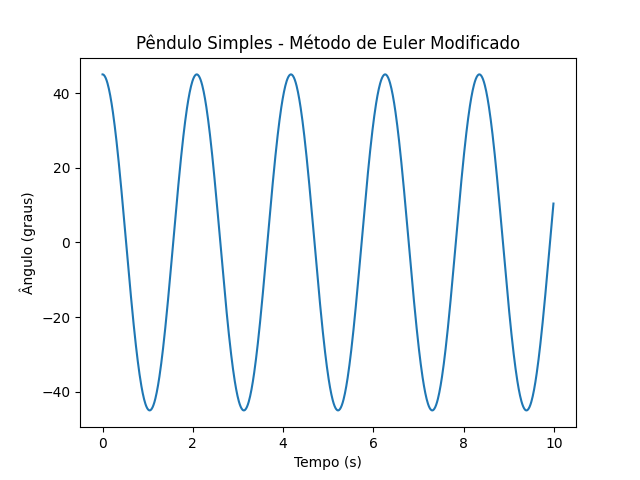
\includegraphics[width=0.5\linewidth]{Figure_PenduloSimplesModificado.png}
    \caption{Movimento do Pêndulo Simples com Euler Modificado.}
    \label{fig:pendulo-modificado}
\end{figure}

\begin{table}[h]
    \centering
    \begin{tabular}{|c|c|c|}
        \hline
        \textbf{Tempo (s)} & \textbf{Ângulo (Graus)} & \textbf{Aceleração Angular (\( \text{Rad/s}^2 \))} \\
        \hline
        0.00 & 45.00 & -6.9296 \\
        0.50 & 2.99 & -0.5104 \\
        1.00 & -44.62 & 6.8841 \\
        1.50 & -8.90 & 1.5164 \\
        2.00 & 43.50 & -6.7463 \\
        \hline
    \end{tabular}
    \caption{Dados de Resultados Adicionais do Pêndulo Simples com Euler Modificado.}
    \label{tab:resultados-adicionais}
\end{table}

Assim, nosso estudo mostra que há métodos mais precisos, algo que será levado em conta em futuras análises.

\section{Conclusão}
Este relatório proporcionou uma abordagem prática à modelagem do pêndulo simples, utilizando LaTeX e métodos numéricos. Os resultados destacam a precisão do modelo. A sensibilidade do método de Euler ressalta a importância da escolha cuidadosa de métodos numéricos.

A combinação de teoria, modelagem e implementação oferece uma perspectiva holística na compreensão de fenômenos físicos. Este trabalho serve como base para estudos futuros de pêndulo duplo.

\begin{thebibliography}{9}
       \bibitem{pendulo-simples}
    João Pedro de Sá Moreira, Eduarda Neves da Silva, Lucas de Oliveira Dalbeto, Mariana de Morais Ribeiro Lião, Amauri Dias Carvalho,
    \emph{ESTUDO E MODELAGEM DE UM PÊNDULO SIMPLES ATRAVÉS DE EQUAÇÕES DIFERENCIAIS E ANÁLISE DE VÍDEO ASSISTIDA POR COMPUTADOR},
    REVISTA ACADÊMICA - ENSINO DE CIÊNCIAS E TECNOLOGIAS, 2019,
    Disponível em: \url{https://www.google.com/url?sa=t&rct=j&q=&esrc=s&source=web&cd=&cad=rja&uact=8&ved=2ahUKEwig5Mm4meyDAxXdLrkGHdFEC4sQFnoECBQQAQ&url=https%3A%2F%2Fintranet.cbt.ifsp.edu.br%2Fqualif%2Fvolume05%2F1.Engenharias%2FEd05_EN_04_37_58.pdf&usg=AOvVaw2CnmAdnInCrznbCjl9aNd7&opi=89978449}.

    \bibitem{Ediciplinas}
    Prof. Alexandre Roma
    Disponível em: \url{https://edisciplinas.usp.br/course/view.php?id=115492}

    \bibitem{GitHub}
    Guilherme Turina, Barbara Bueno
    Disponível em: \url{https://github.com/Turina7/Calculo-Numerico/tree/main}
\end{thebibliography}

\end{document}
